
%%% Local Variables: 
%%% mode: latex
%%% TeX-master: "notes"
%%% End: 

\chapter{Entrada/Saída e Armazenamento}


\def\thetitle{Sistema de arquivos}

\section{\thetitle}

O {\bf sistema de arquivos} é o sistema que obedece uma estrutura
hierárquica específica para armazenamento de dados.

Os sistemas de arquivos normalmente possuem quatro entidades básicas:

\begin{description}
\item{Arquivos: }sequência ordenada de bytes;
\item{Diretórios: }recipiente de arquivos correlacionados ou outros
  diretórios chamados subdiretórios;
\item{Inode: }estrutura de dados separada do arquivo que contém
  atributos a respeito dos arquivos;
\item{Superbloco: }estrutura que contém atributos do sistema de
  arquivos e informações sobre os arquivos.
\end{description}

Os sistemas de arquivos possuem interface de programação comum para
melhorar a portabilidade do sistema. As principais operações são:

\begin{itemize}
\item {\tt open()}\item {\tt read()}\item {\tt write()}
\item {\tt create()}\item {\tt delete()}
\end{itemize}

O funcionamento de cada função depende da entidade à qual a interface
está sendo aplicada.

\subsection{Sistema de arquivos virtual}

O sistema de arquivos virtual implementa a interface entre programas
do espaço do usuário e o sistema de arquivos.

A Figura~\ref{fig:vfs} mostra a chamada de sistema {\tt write()} que é
atendida pelo subsistema de arquivo virtual e utiliza a função
correspondente para o sistema de arquivos em que o meio físico está
formatado para gravação dos dados.

\begin{figure}[h]
  \centering
  
%%% Local Variables: 
%%% mode: latex
%%% TeX-master: "../notes"
%%% End: 


\begin{tikzpicture}
  \tikzset{every node/.style={text centered},
    every edge/.style={->,draw,>=latex}, thelabel/.style={font=\footnotesize}} 
  \footnotesize 
  \node[draw] (w) {{\tt write()}};
  \node[text width=2cm,draw] (vfs) [right of=w,xshift=20mm] {Sistema de
    arquivos virtual};
  \node[shape=circle,minimum size=12mm,draw] (cd) [right of=vfs,
  xshift=25mm] {};
  \node[shape=circle,minimum size=4mm,draw] at (cd) {};
  \node[thelabel] [above of=cd] {CD/DVD};
  \node[shape=cylinder,shape border rotate=90,minimum width=1cm,
  minimum height=1.75cm,draw] (disk) [above of=cd, yshift=15mm]
  {};
  \node[thelabel] [above of=disk,yshift=5mm] {Disco};
  \node[shape=rectangle,minimum width=.75cm,
  minimum height=1.25cm,draw] (pendrive) [below of=cd, yshift=-15mm] {};
  \node[thelabel] [above of=pendrive] {Pendrive};

  %% setas
  \path (w) edge (vfs);
  \path (vfs) edge node[above] {\scriptsize ISO-9660} (cd);
  \path (vfs) edge node[above, rotate=25] {ext3} (disk);
  \path (vfs) edge node[above,rotate=-25] {\scriptsize FAT32} (pendrive);

\end{tikzpicture}  
  \caption{Sistema de arquivos virtual}
  \label{fig:vfs}
\end{figure}

O sistema Microsoft\textsuperscript{$\textregistered$} Windows não
possui sistema de arquivos virtual, portanto somente sistemas de
arquivos que possuem suporte pelo sistema tais como FAT, FAT32 e NTFS
são acessíveis.


A chamada de função 

\begin{tt}
  int ret = write(fd, buf, len);
\end{tt}

representada abstratamente na Figura~\ref{fig:vfs:sys} grava {\tt len}
bytes apontados por {\tt buffer} na posição atual do arquivo
representado pelo descritor de arquivos.

Note que a os dados são repassado para o sistema de arquivos virtual
que se encarrega de distribuir para a função adequada ao sistema de
arquivo no qual se deseja gravar.

\begin{figure}[h]
  \centering
  
%%% Local Variables: 
%%% mode: latex
%%% TeX-master: "../notes"
%%% End: 


\begin{tikzpicture}
  \tikzset{every node/.style={text centered},
    every edge/.style={->,draw,>=latex}, thelabel/.style={font=\footnotesize}} 
  \small \node[draw] (w) {{\tt write()}};
  \node [text width=1cm,below of=w,yshift=-5mm] {\scriptsize Espaço do usuário};
  \node[draw]  (wsys) [right of=w,xshift=15mm] {\tt sys\_write};
  \node [text width=1.5cm,below of=wsys,yshift=-5mm] {\scriptsize Sistema de arquivos virtual};
  \node[text width=2cm,draw]  (fs) [right of=wsys,xshift=20mm] 
  {Função do sistema de arquivos};
  \node [text width=1.5cm,below of=fs,yshift=-5mm] {\scriptsize Sistema de arquivos};
  \node[shape=cylinder,shape border rotate=90,text width=1cm,
  aspect=.5,draw] (disk) [right
  of=fs,xshift=20mm] {Meio físico};

  %% setas
  \path (w) edge (wsys);
  \path (wsys) edge (fs);
  \path (fs) edge (disk);
  

\end{tikzpicture}
  \caption{Fluxo de dados até o meio físico passando pelo sistema de arquivos virtual.}
  \label{fig:vfs:sys}
\end{figure}

\section{Dispositivos de entrada e saída}

Além das abstrações de processos, espaços de endereçamento e arquivos,
os SOs também controlam os dispositivos de E/S para:

\begin{itemize}
\item Emitir comandos para dispositivos;
\item Interceptar interrupções e tratar erros;
\item Atuar como interface entre os dispositivos e o restante do sistema.
\end{itemize}

O dispositivos de E/S podem ser divididos de modo genérico em 3
classes:

\begin{description}
\item[Dispositivos de caractere:] Lidam com fluxo de bytes
  sequenciais, acessadas um byte após o outro. Como exemplo desta
  classe podemos citar o teclado e o mouse, pois a ordem de envio de
  bytes não pode ser alterada.
\item[Dispositivo de bloco:] Lidam com o acesso aleatório
  de ``pedaços'' de dados chamados blocos. Como exemplo temos disco
  rígido, CD/DVD, {\em pendrive}, discos de {\em Blu-ray} e disquete.
\item[Dispositivos de rede:] São os dispositivos que transmitem e
  recebem pacotes de dados. Como exemplo temos a placa de rede.
\end{description}

\subsection{Drivers}

Os {\bf drivers} são módulos com interface de programação bem definida
que ocultam os detalhes de como funciona o dispositivo. O papel do
driver é fornecer {\bf mecanismo} (quais funcionalidades estão
disponíveis) e não {\bf política} (como estas funcionalidade são
utilizadas).

A Figura~\ref{fig:driver} mostra como um kernel monolítico interage
com o driver para fornecer à aplicação acesso às funcionalidade
oferecidas pelo hardware.

\begin{figure}[ht]
  \centering
  
%%% Local Variables: 
%%% mode: latex
%%% TeX-master: "../notes"
%%% End: 


\def\w{2}
\def\h{1.5}
\def\xdelta{1.5}
\def\ydelta{1}
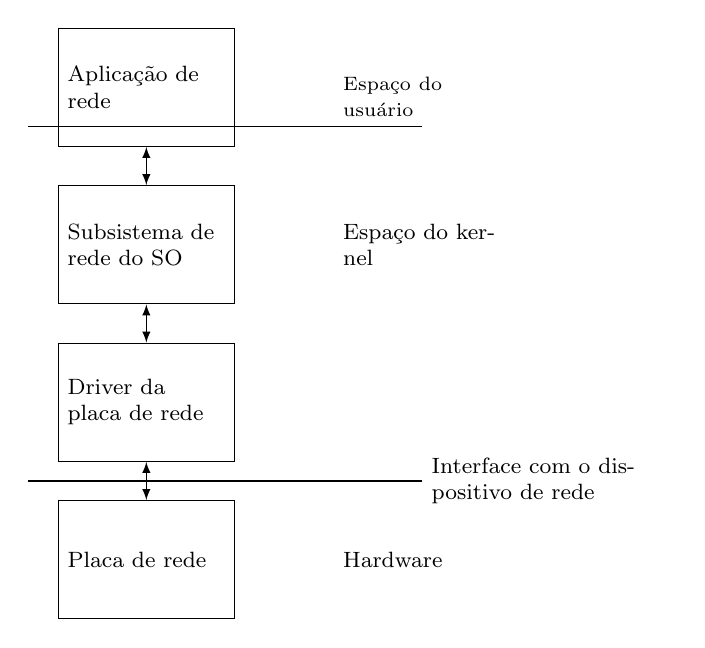
\begin{tikzpicture}
  \tikzset{every node/.style={text width=2cm,font={\footnotesize}},
  module/.style={rectangle,minimum height=1.5cm,draw}}
  \foreach \y/\l in {0/{Aplicação de rede},-2/{Subsistema de rede do
      SO},-4/{Driver da placa de rede},-6/{Placa de rede}} {
    \node[module] (\y) at (0,\y+\h) {\l};
  }
  \foreach \s/\d in {0/-2,-2/-4,-4/-6} {
    \path[<->,>=latex,draw] (\s) -- (\d);
  }

  \draw (-\xdelta,\ydelta) -- (\w+\xdelta,\ydelta) node[above]
  {\scriptsize Espaço
  do usuário};
\node [right of=-2,xshift=25mm] {Espaço do kernel};

  \draw (-\xdelta,-3.5) -- (\w+\xdelta,-3.5) node[text width=3cm,right] {Interface com o
    dispositivo de rede};
  \node [right of=-6,xshift=25mm] {Hardware};
\end{tikzpicture}  
  \caption{Fluxo de dados da aplicação até o hardware passando pelo sistema (kernel) e driver.}
  \label{fig:driver}
\end{figure}

